\chapter{Preparação Dos Dados}
Muitos dos métodos existentes para detecção de botnets, utilizam informações completas do tráfego da rede, inclusive de informações do \textit{payload} para extrair as características relevantes \citep{krmicek2011inspecting}. Infelizmente, nem sempre todas essas informações estão presentes, por diversos motivos, como questões de privacidade ou falta de autorização para acessar o conteúdo dos pacotes. Por isso, torna-se necessário analisar a capacidade de utilizar informações mais simples, como o fluxo da rede (\textit{NetFlow}) ou o registro do log de requisições a um servidor DNS, para características.

Nesse trabalho vamos focar nos dados das requisições coletadas pelo servidor DNS do IME no período de fevereiro a abril de 2012. Ao longo desse capítulo mostraremos quais as informações contidas nesses registros, as características que consideramos relevantes e como foi feito o tratamento para a extração das mesmas.

\section{Estrutura do Log Bruto de DNS }
O log de DNS utilizado foi baseado nos dados coletados pelo servidor DNS do IME. Esses dados são privados e foram coletados em diversos dias de fevereiro a abril de 2012. Cada registro no DNS é uma requisição que foi feita ao servidor por uma máquina cliente. As informações contidas em cada registro são:

\begin{itemize}
\item Data em que a requisição foi feita
\item Horário com precisão de milésimos da requisição
\item Endereço IP da máquina que fez a requisição
\item Porta do Cliente
\item Nome do domínio requisitado
\item Tipo de Requisição
\item IP do Servidor DNS consultado
\end{itemize}

Abaixo, encontra-se um exemplo de uma entrada no registro de requisições extraído da base de dados: 

\begin{quote}
11-Mar-2012 12:24:16.772 queries: info: client 41.128.225.42\#57135: query: rEcREIo.DE9.iMe.eb.br IN A - (200.20.120.33)
\end{quote}

Dado que os dados não estão estruturados em um formato facilmente reconhecido pelo computador, como em um arquivo JSON ou XML, foi preciso realizar a extração dos dados do log utilizando expressões regulares. A expressão regular foi construída inicialmente para reconhecer alguns exemplos de entradas. Após isso, ela foi aperfeiçoada para reconhecer novos exemplos ao colocar um mecanismo para que o sistema avise quando a entrada não foi reconhecida pela expressão regular. Dessa forma, a expressão era adaptada para reconhecer entradas válidas e que não forem reconhecidas. O mecanismo de aviso foi mantido, afim de garantir o aviso ao usuário de entradas no log que não foram previstas pela expressão regular desenvolvida.

Após aplicar a expressão regular em cada linha extraída do log do servidor DNS do IME, foram filtradas as requisições que foram feitas por máquinas que pertencem à infra-estrutura do IME, como o servidor de correio, já que são seguras e muitas vezes responsáveis por mais de 50\% das entradas no log nos dias analisados. Depois de aplicar esse filtro, o dado tratado pode ser armazenado de modo amigável para a criação do modelo.

\section{A Estrutura do Banco de Dados}
Apenas conseguir fazer a leitura de cada campo do log individualmente não é o suficiente para representar as características que serão utilizadas pelos algoritmos de aprendizado de máquina. Ou seja, elas ainda precisam ser submetidas a diversos cálculos e tratamentos. Com o objetivo de acelerar o processamento desses tratamentos, além de facilitar e agilizar a consulta de informações posteriormente para efetuar uma investigação inicial dos suspeitos levantados pelo sistema, decidimos armazenar as informações em um banco de dados relacional.

O Sistema Gerenciador de Banco de Dados utilizado foi o PostgreSQL, como parte da nossa solução, para facilitar a escrita, leitura e atualização das informações coletadas dos registros DNS. Na modelagem feita, utilizou-se três tabelas para representar as informações contidas no log. A figura \ref{fig:relational_diagram} apresenta a representação relacional do banco de dados, no qual já está incluso as características a serem analisadas como será esclarecido na sessão Levantamento das Características. Dessas três tabelas, a mais importante é a \textit{clients}, pois essa é a que realmente será utilizada pelos algoritmos de aprendizado de máquina. As tabelas \textit{dns\_queries} e \textit{domains} tem função apenas de auxiliar o cálculo da tabela \textit{clients}, porém podem servir também para consultas, caso alguém deseje utilizar a base de dados construídas para inspeção manual posterior.

\begin{figure}
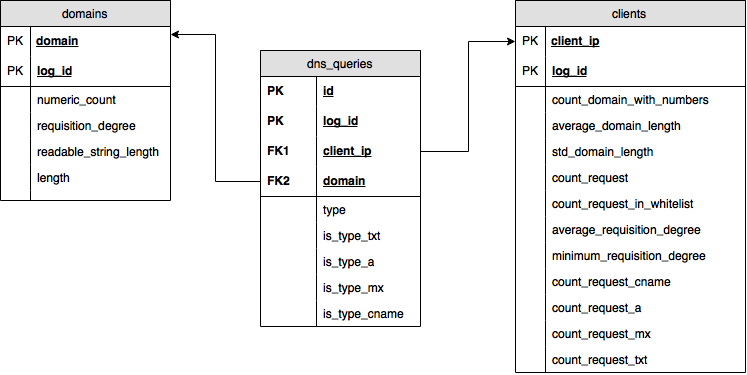
\includegraphics[width=\textwidth]{relational_diagram}
\caption[Diagrama Relacional do Sistema]{Diagrama Relacional do Sistema} \label{fig:relational_diagram}
\end{figure}

A tabela \textit{dns\_queries} é a que melhor representa a estrutura bruta do log de DNS. Mesmo sendo simples, sem muitos tratamentos, ela já apresenta consultas interessantes, como verificar que domínios uma máquina consultou. Os campos \textit{is\_type\_a}, \textit{is\_type\_mx}, \textit{is\_type\_cname}, \textit{is\_type\_txt} são booleanos e indicam apenas se o domínio é do tipo especificado. Embora essa informação já esteja presente na coluna \textit{type}, eles foram adicionados para facilitar cálculos posteriores. A Figura \ref{fig:dns_queries} mostra exemplos de algumas entradas nessa tabela, o cálculo da coluna \textit{query\_time} ainda não foi implementado.

\begin{figure}
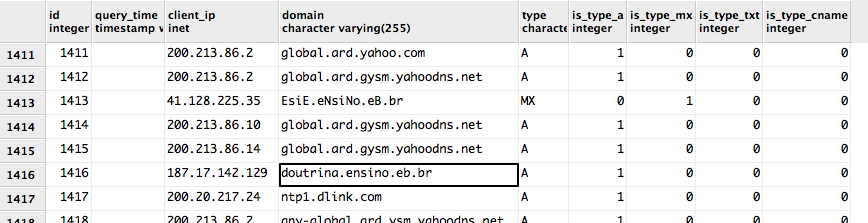
\includegraphics[width=\textwidth]{dns_queries}
\caption[Exemplos de entradas na tabela \textit{dns\_queries}]{Exemplos de entradas na tabela \textit{dns\_queries}} \label{fig:dns_queries}
\end{figure}

A tabela \textit{domains} contém informações referentes à cada domínio consultado. A coluna \textit{length} representa a quantidade de caracteres presentes no nome do domínio. A coluna \textit{numeric\_count} contém a informação de quantos caracteres numéricos estão presentes no domínio. A coluna \textit{readable\_string\_length} calcula a maior \textit{substring} legível do domínio, porém essa coluna não foi utilizada posteriormente, já que o ideal seria calcular o tamanho total legível da \textit{string}, mas devido a complexidade desse cálculo  ele não foi utilizado. A coluna \textit{is\_in\_whitelist} verifica se o domínio está na \textit{whitelist} utilizada, porém verificou-se que muitos domínios consultados conhecidos não estavam lá, abrindo margem para aprimoramento ao incrementar a \textit{whitelist} utilizada para o cenário do Exército Brasileiro. Finalmente, a coluna \textit{requisition\_degree} é bem interessante, informando o grau de requisição do domínio, ou seja, quantas máquinas diferentes também consultaram esse domínio. A Figura \ref{fig:domains} mostra exemplos de algumas entradas nessa tabela, o cálculo das colunas \textit{is\_suspect} e \textit{alexa\_degree} ainda não foi implementado.

\begin{figure}
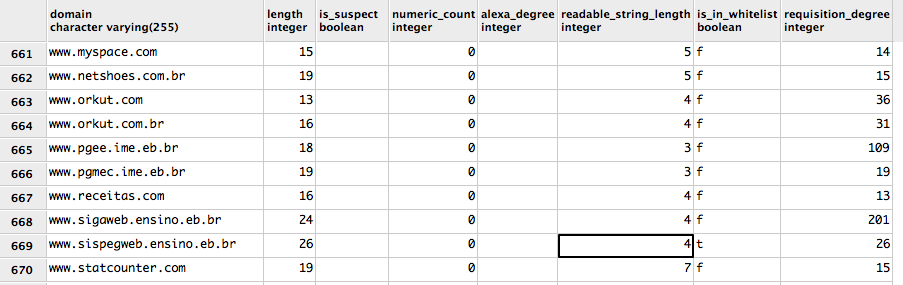
\includegraphics[width=\textwidth]{domains}
\caption[Exemplos de entradas na tabela \textit{domains}]{Exemplos de entradas na tabela \textit{domains}} \label{fig:domains}
\end{figure}

A tabela \textit{clients} representa as máquinas que fizeram requisições DNS no período de tempo analisado, sendo assim, ela é a mais importante para os algoritmos de aprendizado, já que o sistema está preocupado em descobrir as máquinas infectadas. O cálculo das colunas é feito com o auxílio das tabelas \textit{domains} e \textit{dns\_queries}, que guardam a informação de como o cliente tem se comportado na rede. Suas colunas são basicamente as características que são analisadas na seção seguinte. Na figura \ref{fig:clients} são mostrados alguns valores para essas colunas. Devido ao elevado número de colunas nessa tabela, algumas delas foram omitidas para melhorar a visualização.

\begin{figure}
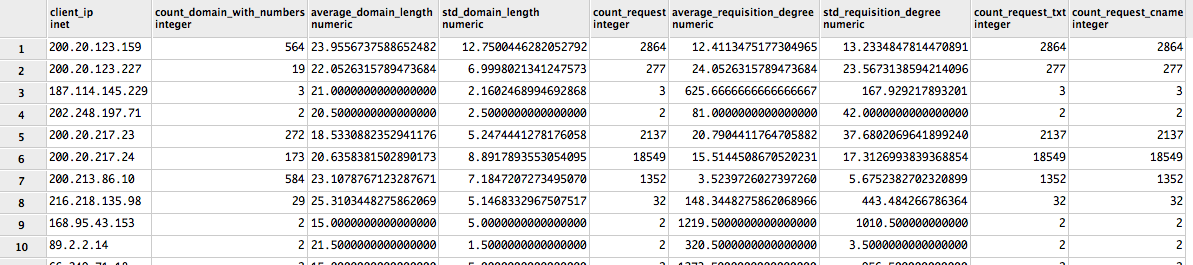
\includegraphics[width=\textwidth]{clients}
\caption[Exemplos de entradas na tabela \textit{clients}]{Exemplos de entradas na tabela \textit{clients}} \label{fig:clients}
\end{figure}

\section{Levantamento das Características}
De posse das informações apresentadas nos capítulos anteriores, é possível definir mais claramente o problema que esse trabalho se propõe a resolver e, em linhas gerais, como ele será abordado.

O objetivo desse trabalho é a partir das informações obtidas no log de registros de um servidor DNS, acusar quais máquinas na rede são suspeitas de pertencer a uma botnet e merecem atenção para uma investigação mais profunda. Para isso, foram pensadas características que uma máquina pertencente a uma botnet pode exibir que a distingue de uma máquina com uso normal.

As características analisadas foram divididas em quatro tipos, que identificam comportamentos divergentes do uso comum que esperam ser observados: a forma de escolha dos domínios, o comportamento de máquina, os domínios visitados em comum e tipos de requisição.

\subsection{Escolha dos Domínios}
Muitas botnets utilizam técnicas de geração de domínio \citep{zhou2013dga}. Essa técnica permite que os bots consultem um grande conjunto de domínios a procura do C\&C, porém apenas um pequeno conjunto desses domínios são de fato utilizados. Essa prática gera nomes não legíveis, muitas vezes formados apenas por números e palavras não legíveis. Além disso, por conveniência, é possível que os domínios gerados por uma mesma botnet tenham o mesmo número de caracteres. Por outro lado, apenas 7.3\% dos domínios dos um milhão primeiros domínios da Alexa contem número e que o tamanho do domínio de um usuário comum não segue nenhum padrão específico.

Não há garantia que essa feature é sempre efetiva, dado que o atacante pode gerar domínios de tamanho variável e evitar números ao gerar o domínio, por isso após a realização dos experimentos será possível confirmar ou não essa hipótese.

Para explorar essas propriedades foram propostas as seguintes características 

\begin{itemize}
\item Quantidade de consultas a domínios com números 
\item Média do comprimento de domínios consultados
\item Desvio Padrão dos comprimentos dos domínios consultados
\end{itemize}

\subsection{Comportamento de Máquina}

O tempo de reação de um humano a uma requisição sem sucesso não pode ser de décimos de segundo, por mera limitação de reflexo. Qualquer sinal de uso que apresente um baixo intervalo entre consultas, algo que apenas uma máquina pode fazer, deve ser considerada suspeita. Além disso, é possível que a máquina acabe por visitar uma quantidade de domínios maior do que o normal ou faça consultas em intervalos regulares, pré-programados, coisa que um ser humano normal raramente irá realizar. Novamente, esse tipo de feature precisa ser validado, pois o comportamento de máquina pode ser mascarado, ao configurar um intervalo aleatório entre consultas e com um certo atraso.

Para explorar essas propriedades foram propostas as seguintes características 

\begin{itemize}
\item Média do intervalo entre as consultas
\item Desvio padrão dos intervalos entre consultas
\item Quantidade total de consultas realizadas
\end{itemize}

\subsection{Domínio Visitados em Comum}
Espera-se que domínios suspeitos sejam acessados apenas por poucas máquinas, como os domínios gerados por algoritmos de geração de domínios para tentar estabelecer uma comunicação com o C\&C. Devido a isso, espera-se que os bots tentem acessar domínios que dificilmente serão procurados por máquinas normais, além do que, se a máquina infectada procura o centro de comando e controle, espera-se que muito dos domínios consultados por ela também sejam dessa forma, ou seja pouco procurado por outras máquinas.

Para analisar essa propriedade, foi necessário realizar um pré-processamento, que analisa para cada domínio consultado, por quantas máquinas diferentes ele foi consultado. Essa quantidade de máquinas que requisitou um domínio específico chamaremos de grau de requisição do domínio.

Dessa forma, acredita-se que as informações relativas ao grau dos domínios consultados pela máquina podem ser úteis para identificar um comportamento suspeito em uma máquina. Foram levantadas as seguintes características:

\begin{itemize}
\item Grau de requisição mínimo entre os graus dos domínios consultados pela máquina
\item Média dos graus de requisição dos domínios consultados pela máquina
\item Desvio Padrão dos graus de requisição dos domínios consultados pela máquina

\end{itemize}

\subsection{Tipos de Requisição}

Não se tem informação sobre máquinas seguindo padrão quanto ao tipo de requisição DNS solicitadas. Porém, esse dado é de fácil acesso e seu estudo pode evidenciar a exploração de alguma fragilidade ainda não analisada nas requisições DNS. Por exemplo, os registros do tipo TXT raramente são utilizados atualmente para leitura de seres humanos. Para isso levantamos algumas características quanto ao tipos de requisição DNS realizadas:

\begin{itemize}
\item Quantidade de consultas do tipo A (Registro de Endereço) realizadas
\item Porcentagem de consultas do tipo A realizadas
\item Quantidade de consultas do tipo MX (Registro de Troca de Mensagens) realizadas
\item Porcentagem de consultas do tipo MX realizadas
\item Quantidade de consultas do tipo CNAME (Nome Canônico) realizadas
\item Porcentagem de consultas do tipo CNAME realizadas
\item Quantidade de consultas do tipo TXT (Registro de Texto) realizadas
\item Porcentagem de consultas do tipo TXT realizadas
\end{itemize}

Com essas informações calculadas, é possível submeter as informações contidas no log de DNS para serem tratadas por algoritmos de agrupamento. Espera-se que os bots apresentem comportamento diferente de usuários normais, seguindo padrões que não são seguidos por usuários normais, fazendo com que eles fiquem agrupados em grupos menores, que devem ser investigados.
